\documentclass{article}
\usepackage[utf8]{inputenc}
\usepackage{indentfirst}
\usepackage{amsmath}
\usepackage{amsthm}
\usepackage{graphicx}
\usepackage{float}
\title{RL Crash Course + Some Thoughts}
\author{Ding (Eric) Ding}
\date{November 2022}
\begin{document}

\maketitle

\section{Introduction}
    In this Project, I followed OpenAI deep reinforcement learning course, and used Spinning Up for exercises and experiments.

\section{What's Omitted}
    Regularization, Observation normalization

\section{Key Concepts}
    The main characters of RL are the agent and the environment. The environment is the world that the agent lives in and interacts with. At every step of interaction, the agent sees a (possibly partial) observation of the state of the world, and then decides on an action to take. The environment changes when the agent acts on it, but may also change on its own.
    \begin{figure}[H]
        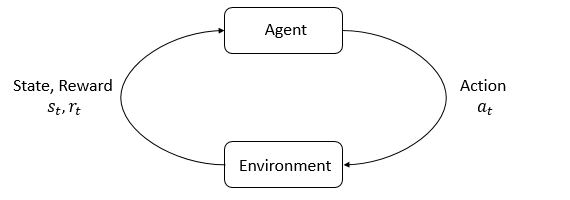
\includegraphics[width=\linewidth]{rl_diagram_transparent_bg.png}
        \caption{RL framework}
        \label{fig:rl}
      \end{figure}

    The agent also perceives a reward signal from the environment, a number that tells it how good or bad the current world state is. The goal of the agent is to maximize its cumulative reward, called return. Reinforcement learning methods are ways that the agent can learn behaviors to achieve its goal.

    States and observations: represented by matrix

    Action Spaces: the set of all valid actions. Discrete / continuous.

    Policies: a rule used by an agent to decide what actions to take. Deterministic: $a_t = \mu_{\theta}(s_t)$. Stochastic: $a_t \approx \pi_{\theta}(\cdot | s_t)$. In deep RL, we deal with parametrized policies, with parameters that can be adjusted by optimization.

\section{Ideas}
    \subsection{Observation}
      Fully observed environment vs. partially observed\
    \subsection{Action}
      Rule out certain actions in action space

\end{document}